\documentclass[11pt,a4paper]{report}
\usepackage[textwidth=37em,vmargin=30mm]{geometry}
\usepackage{calc,xunicode,amsmath,amssymb,paralist,enumitem,tabu,booktabs,datetime2,xeCJK,xeCJKfntef,listings}
\usepackage{tocloft,fancyhdr,tcolorbox,xcolor,graphicx,eso-pic,xltxtra,xelatexemoji}

\newcommand{\envyear}[0]{2025}
\newcommand{\envdatestr}[0]{2025-04-10}
\newcommand{\envfinaldir}[0]{webdb/2025/20250410/final}

\usepackage[hidelinks]{hyperref}
\hypersetup{
    colorlinks=false,
    pdfpagemode=FullScreen,
    pdftitle={Web Digest - \envdatestr}
}

\setlength{\cftbeforechapskip}{10pt}
\renewcommand{\cftchapfont}{\rmfamily\bfseries\large\raggedright}
\setlength{\cftbeforesecskip}{2pt}
\renewcommand{\cftsecfont}{\sffamily\small\raggedright}

\setdefaultleftmargin{2em}{2em}{1em}{1em}{1em}{1em}

\usepackage{xeCJK,xeCJKfntef}
\xeCJKsetup{PunctStyle=plain,RubberPunctSkip=false,CJKglue=\strut\hskip 0pt plus 0.1em minus 0.05em,CJKecglue=\strut\hskip 0.22em plus 0.2em}
\XeTeXlinebreaklocale "zh"
\XeTeXlinebreakskip = 0pt


\setmainfont{Brygada 1918}
\setromanfont{Brygada 1918}
\setsansfont{IBM Plex Sans}
\setmonofont{JetBrains Mono NL}
\setCJKmainfont{Noto Serif CJK SC}
\setCJKromanfont{Noto Serif CJK SC}
\setCJKsansfont{Noto Sans CJK SC}
\setCJKmonofont{Noto Sans CJK SC}

\setlength{\parindent}{0pt}
\setlength{\parskip}{8pt}
\linespread{1.15}

\lstset{
	basicstyle=\ttfamily\footnotesize,
	numbersep=5pt,
	backgroundcolor=\color{black!5},
	showspaces=false,
	showstringspaces=false,
	showtabs=false,
	tabsize=2,
	captionpos=b,
	breaklines=true,
	breakatwhitespace=true,
	breakautoindent=true,
	linewidth=\textwidth
}






\newcommand{\coverpic}[2]{
    % argv: itemurl, authorname
    Cover photo by #2~~(\href{#1}{#1})
}
\newcommand{\makeheader}[0]{
    \begin{titlepage}
        % \newgeometry{hmargin=15mm,tmargin=21mm,bmargin=12mm}
        \begin{center}
            
            \rmfamily\scshape
            \fontspec{BaskervilleF}
            \fontspec{Old Standard}
            \fontsize{59pt}{70pt}\selectfont
            WEB\hfill DIGEST
            
            \vfill
            % \vskip 30pt
            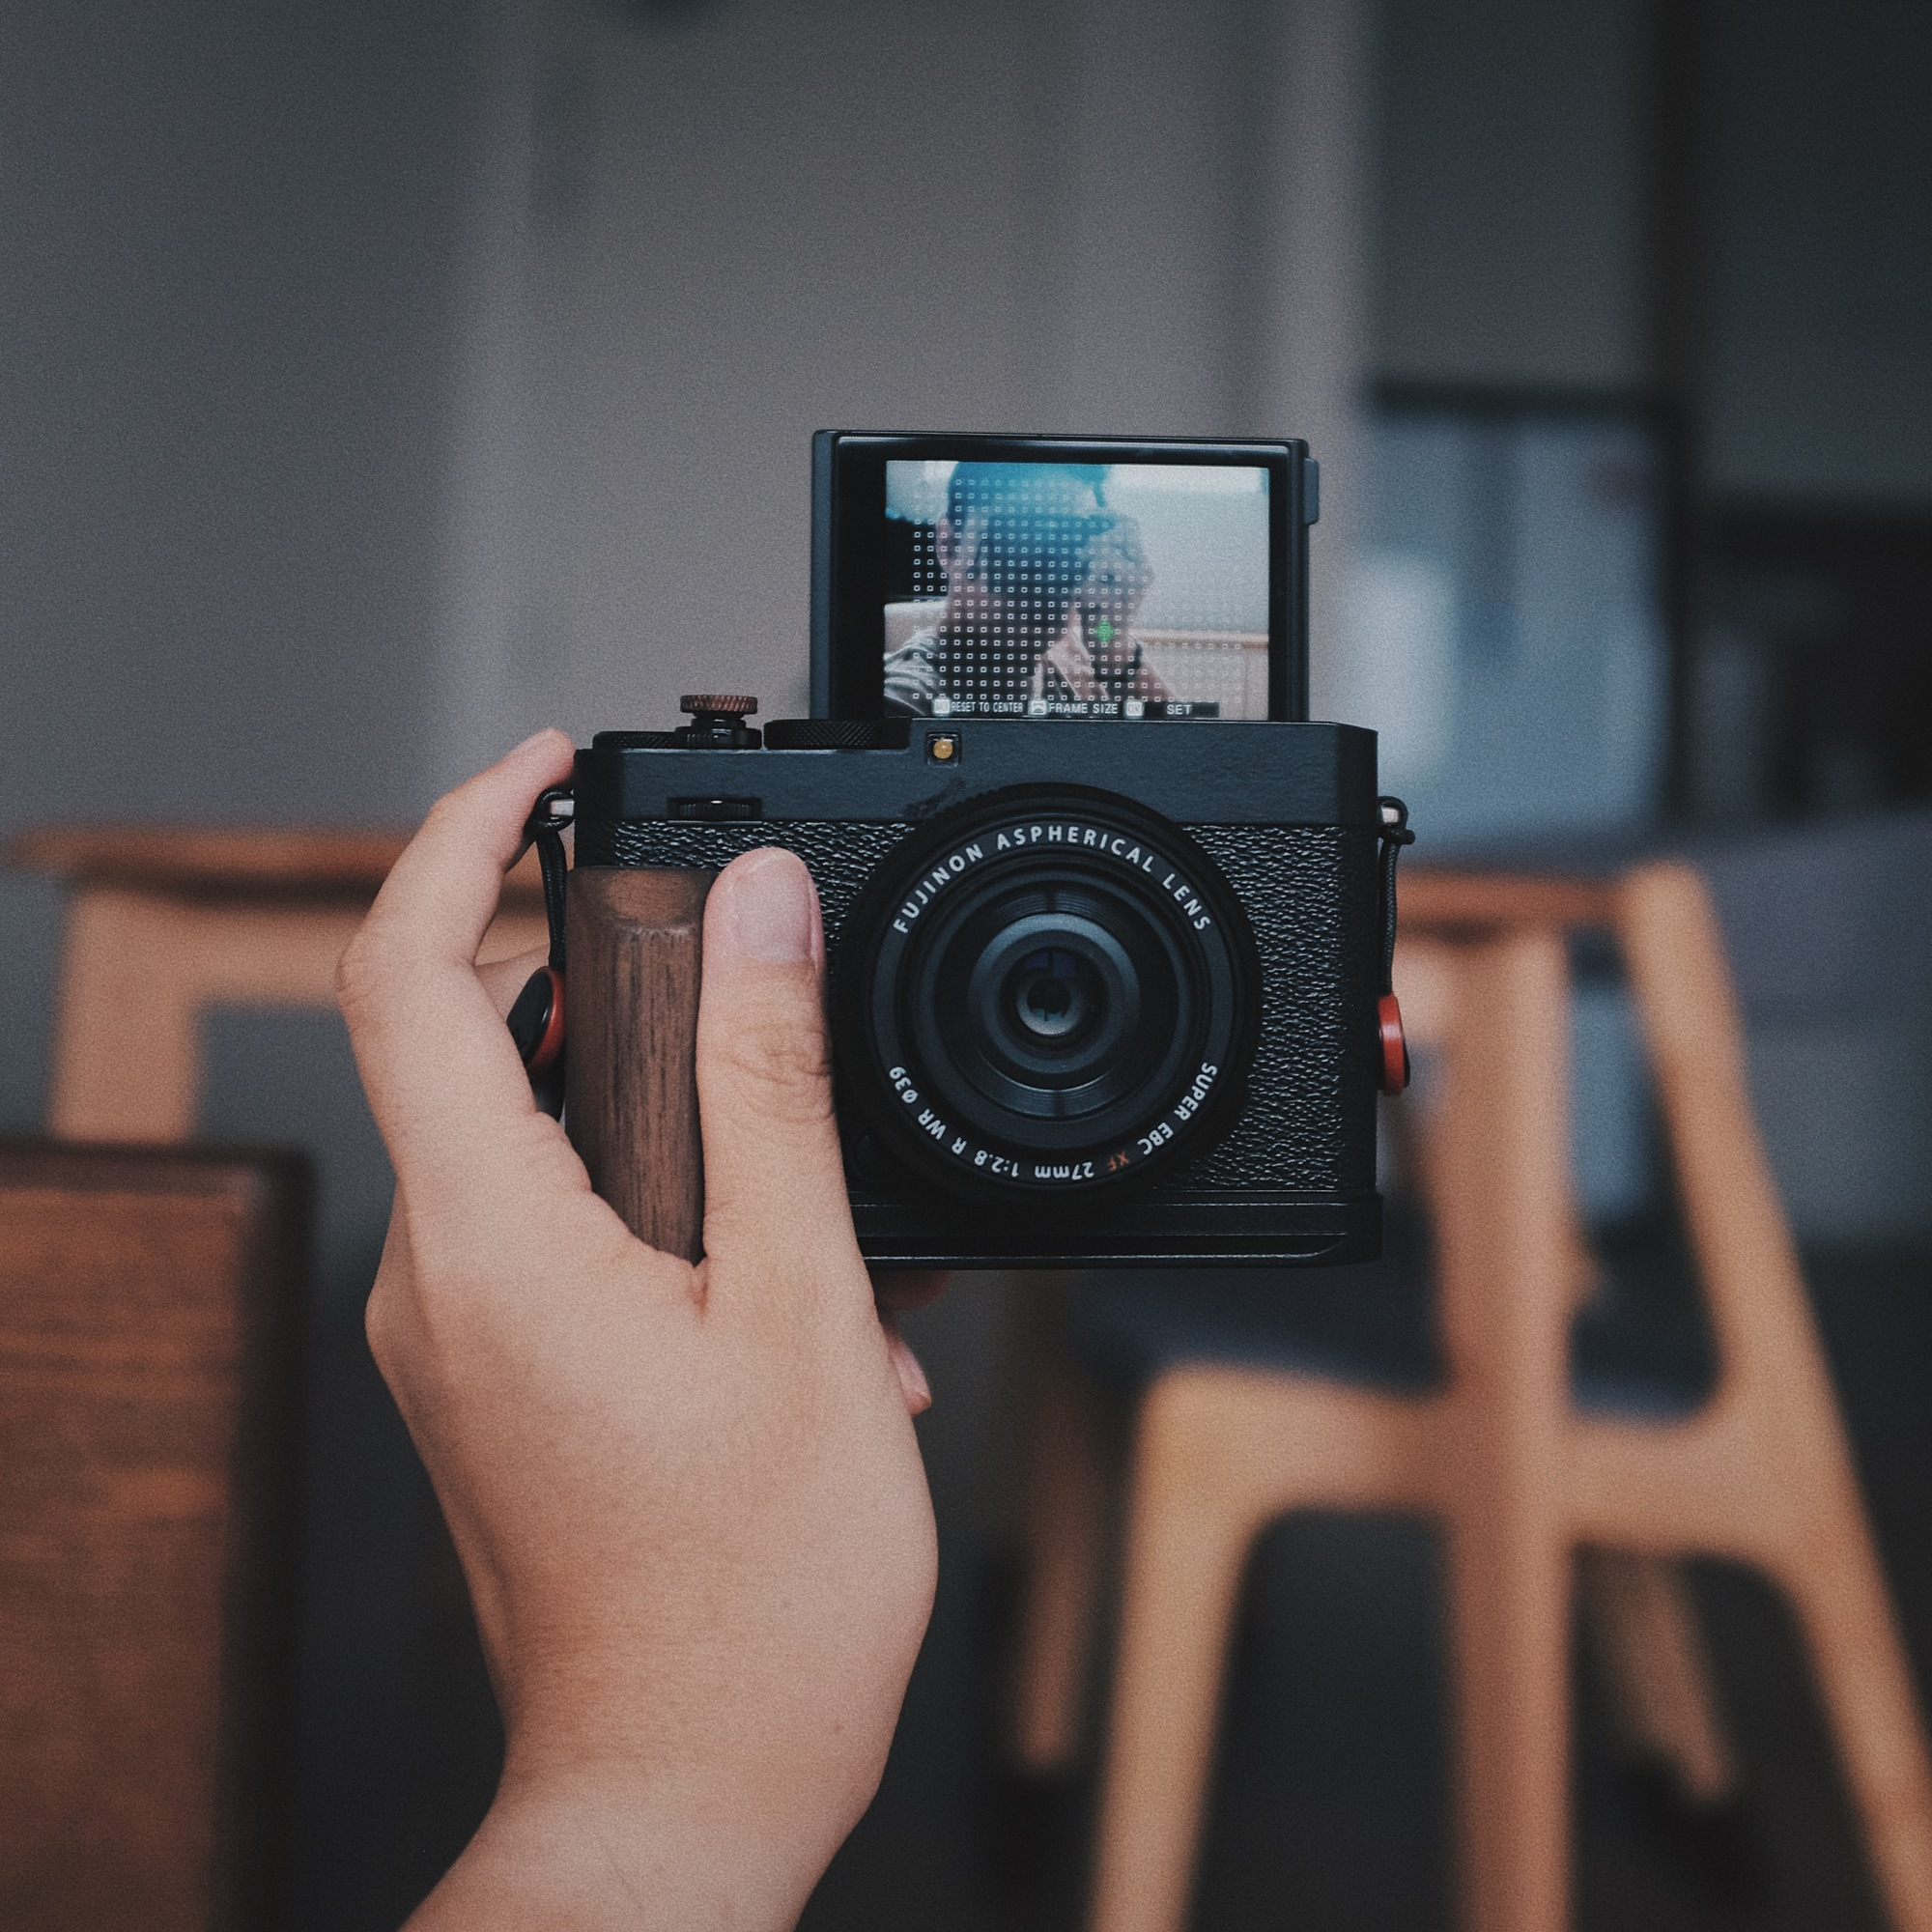
\includegraphics[width=\linewidth]{\envfinaldir/coverpic-prod.jpg}\par
            % \vskip 30pt
            \vfill

            \normalsize\rmfamily\scshape
            \copyright{} The Web Digest Project \hfill\large \envdatestr
        \end{center}
    \end{titlepage}
    % \restoregeometry
}
\newcommand{\simplehref}[1]{%
    \textcolor{blue!80!green}{\href{#1}{#1}}%
}
\renewcommand{\contentsname}{\center\Huge\sffamily\bfseries Contents\par\vskip 20pt}
\newcounter{ipartcounter}
\setcounter{ipartcounter}{0}
\newcommand{\ipart}[1]{
    % \vskip 20pt
    \clearpage
    \stepcounter{ipartcounter}
    \phantomsection
    \addcontentsline{toc}{chapter}{#1}
    % \begin{center}
    %     \Huge
    %     \sffamily\bfseries
    %     #1
    % \end{center}
    % \vskip 20pt plus 7pt
}
\newcounter{ichaptercounter}
\setcounter{ichaptercounter}{0}
\newcommand{\ichapter}[1]{
    % \vskip 20pt
    \clearpage
    \stepcounter{ichaptercounter}
    \phantomsection
    \addcontentsline{toc}{section}{\numberline{\arabic{ichaptercounter}}#1}
    \begin{center}
        \Huge
        \sffamily\bfseries
        #1
    \end{center}
    \vskip 20pt plus 7pt
}
\newcommand{\entrytitlefont}[1]{\subsection*{\raggedright\Large\sffamily\bfseries#1}}
\newcommand{\entryitemGeneric}[2]{
    % argv: title, url
    \parbox{\linewidth}{
        \entrytitlefont{#1}\par\vskip 5pt
        \footnotesize\ttfamily\mdseries
        \simplehref{#2}
    }\vskip 11pt plus 11pt minus 1pt
}
\newcommand{\entryitemGithub}[3]{
    % argv: title, url, desc
    \parbox{\linewidth}{
        \entrytitlefont{#1}\par\vskip 5pt
        \footnotesize\ttfamily\mdseries
        \simplehref{#2}\par\vskip 5pt
        \small\rmfamily\mdseries#3
    }\vskip 11pt plus 11pt minus 1pt
}
\newcommand{\entryitemAp}[3]{
    % argv: title, url, desc
    \parbox{\linewidth}{
        \entrytitlefont{#1}\par\vskip 5pt
        \footnotesize\ttfamily\mdseries
        \simplehref{#2}\par\vskip 5pt
        \small\rmfamily\mdseries#3
    }\vskip 11pt plus 11pt minus 1pt
}
\newcommand{\entryitemHackernews}[3]{
    % argv: title, hnurl, rawurl
    % \parbox{\linewidth}{
    %     \entrytitlefont{#1}\par\vskip 5pt
    %     \footnotesize\ttfamily\mdseries
    %     \simplehref{#3}\par
    %     \textcolor{black!50}{\href{#2}{#2}}
    % }\vskip 11pt plus 11pt minus 1pt
    \begin{minipage}{\linewidth}
            \entrytitlefont{#1}\par\vskip 5pt
            \footnotesize\ttfamily\mdseries
            \simplehref{#3}\par
            \textcolor{black!50}{\href{#2}{#2}}
    \end{minipage}\par\vskip 11pt plus 11pt minus 1pt
}







\begin{document}

\makeheader

\tableofcontents\clearpage




\ipart{Developers}
\ichapter{Hacker News}
\entryitemTwoLinks{Basic Income Pilot Project: Study results}{https://news.ycombinator.com/item?id=43636757}{https://www.pilotprojekt-grundeinkommen.de/en}

\entryitemTwoLinks{Claude's Max Plan}{https://news.ycombinator.com/item?id=43635296}{https://www.anthropic.com/news/max-plan}

\entryitemTwoLinks{GPD Pocket 4 Speaker DSP: Configuring PipeWire so laptop speakers sound better}{https://news.ycombinator.com/item?id=43635295}{https://kittenlabs.de/blog/2025/04/06/gpd-pocket-4-speaker-dsp/}

\entryitemTwoLinks{Trump temporarily drops tariffs to 10\% for most countries}{https://news.ycombinator.com/item?id=43634806}{https://www.cnbc.com/2025/04/09/trump-announces-90-day-tariff-pause-for-at-least-some-countries.html}

\entryitemTwoLinks{DOJ will no longer prosecute cryptocurrency fraud}{https://news.ycombinator.com/item?id=43634582}{https://www.theverge.com/policy/645399/trump-doj-cryptocurrency-fraud-prosecutions-memo}

\entryitemTwoLinks{How University Students Use Claude}{https://news.ycombinator.com/item?id=43633383}{https://www.anthropic.com/news/anthropic-education-report-how-university-students-use-claude}

\entryitemTwoLinks{Show HN: I built an app to generate story relationships using Mermaidjs}{https://news.ycombinator.com/item?id=43633298}{https://github.com/herol3oy/austen}

\entryitemTwoLinks{The chroot Technique – a Swiss army multitool for Linux systems}{https://news.ycombinator.com/item?id=43632379}{https://livesys.se/posts/the-chroot-technique/}

\entryitemTwoLinks{SpacetimeDB}{https://news.ycombinator.com/item?id=43631822}{https://spacetimedb.com/}

\entryitemTwoLinks{Man pages are great, man readers are the problem}{https://news.ycombinator.com/item?id=43631672}{https://whynothugo.nl/journal/2025/04/09/man-pages-are-great-man-readers-are-the-problem/}

\entryitemTwoLinks{Quality-of-Life in Tetris Games}{https://news.ycombinator.com/item?id=43631656}{https://jcarlosroldan.com/post/355}

\entryitemTwoLinks{How much do you think it costs to make a pair of Nike shoes in Asia?}{https://news.ycombinator.com/item?id=43631543}{https://threadreaderapp.com/thread/1909741170953273353.html}

\entryitemTwoLinks{Tesla Solar Sales Declined for 4 Qtrs. Then Tesla Stopped Publishing the Numbers}{https://news.ycombinator.com/item?id=43631402}{https://cleantechnica.com/2025/04/07/tesla-solar-sales-declined-for-4-straight-quarters-then-tesla-stopped-publishing-the-numbers/}

\entryitemTwoLinks{Fake job seekers are flooding US companies that are hiring for remote positions}{https://news.ycombinator.com/item?id=43631384}{https://www.cnbc.com/2025/04/08/fake-job-seekers-use-ai-to-interview-for-remote-jobs-tech-ceos-say.html}

\entryitemTwoLinks{The Agent2Agent Protocol (A2A)}{https://news.ycombinator.com/item?id=43631381}{https://developers.googleblog.com/en/a2a-a-new-era-of-agent-interoperability/}

\entryitemTwoLinks{American Disruption}{https://news.ycombinator.com/item?id=43631276}{https://stratechery.com/2025/american-disruption/}

\entryitemTwoLinks{Ironwood: The first Google TPU for the age of inference}{https://news.ycombinator.com/item?id=43631274}{https://blog.google/products/google-cloud/ironwood-tpu-age-of-inference/}

\entryitemTwoLinks{Photographs of 19th Century Japan}{https://news.ycombinator.com/item?id=43631251}{https://cosmographia.substack.com/p/photographs-of-old-japan}

\entryitemTwoLinks{Whisky is no longer actively maintained}{https://news.ycombinator.com/item?id=43631230}{https://docs.getwhisky.app/maintenance-notice}

\entryitemTwoLinks{How to lock down your phone if you're traveling to the U.S.}{https://news.ycombinator.com/item?id=43630624}{https://www.washingtonpost.com/technology/2025/03/27/cbp-cell-phones-devices-traveling-us/}\ichapter{Phoronix}
\entryitemGeneric{\hskip 0pt{}TUXEDO Provides Update On Their Snapdragon X Elite Linux Laptop}{https://www.phoronix.com/news/TUXEDO-Snapdragon-Laptop-Update}

\entryitemGeneric{\hskip 0pt{}Framework Laptop 12 Pre-Orders Open, Starting At €569}{https://www.phoronix.com/news/Framework-12-Pre-Orders-Open}

\entryitemGeneric{\hskip 0pt{}AMD Prepping PKI Accelerator Driver "AMDPK" For Linux}{https://www.phoronix.com/news/AMD-PKI-Accelerator-AMDPK-Linux}

\entryitemGeneric{\hskip 0pt{}AMD To Detail ROCm Open-Source Software Progress In June}{https://www.phoronix.com/news/AMD-ROCm-June-2025-Announcement}

\entryitemGeneric{\hskip 0pt{}OpenSSH 10.0 Released To Better Fend Off Attacks By Quantum Computers}{https://www.phoronix.com/news/OpenSSH-10.0-Released}

\entryitemGeneric{\hskip 0pt{}Benchmarks: Google Cloud's New C4D VMs Deliver Remarkable Performance With AMD EPYC Turin}{https://www.phoronix.com/review/google-c4d-amd-epyc-turin}

\entryitemGeneric{\hskip 0pt{}Ubuntu 25.04 Now Ships With JPEG-XL Support Enabled By Default}{https://www.phoronix.com/news/Ubuntu-25.04-JPEG-XL-Default}

\entryitemGeneric{\hskip 0pt{}RadeonSI Driver Wires Up Support For 16-bit NIR Types: Benefits GLES \& OpenCL}{https://www.phoronix.com/news/RadeonSI-16-bit-NIR-Types}

\entryitemGeneric{\hskip 0pt{}Initial Support For Apple Cores Merged For The GCC 15 Compiler: A12, M1, M2 \& M3}{https://www.phoronix.com/news/GCC-15-Merges-Apple-Cores}\ichapter{Dribbble}
\entryitemGeneric{\hskip 0pt{}Fintech Web Design \& Landing Page for Puzzle}{https://dribbble.com/shots/25652139-Fintech-Web-Design-Landing-Page-for-Puzzle}

\entryitemGeneric{\hskip 0pt{}Hawkridge}{https://dribbble.com/shots/25877367-Hawkridge}

\entryitemGeneric{\hskip 0pt{}Nite Riot®\_Film Production // Case Study\_Vol.1.0}{https://dribbble.com/shots/25874978-Nite-Riot-Film-Production-Case-Study-Vol-1-0}

\entryitemGeneric{\hskip 0pt{}UltraSlot}{https://dribbble.com/shots/25875506-UltraSlot}

\entryitemGeneric{\hskip 0pt{}Sidekick Ai 3d mascot}{https://dribbble.com/shots/25874949-Sidekick-Ai-3d-mascot}

\entryitemGeneric{\hskip 0pt{}Howzit}{https://dribbble.com/shots/25871668-Howzit}

\entryitemGeneric{\hskip 0pt{}Brainstorm}{https://dribbble.com/shots/25871145-Brainstorm}

\entryitemGeneric{\hskip 0pt{}Boxplates}{https://dribbble.com/shots/25869902-Boxplates}

\entryitemGeneric{\hskip 0pt{}Nord Print Logo Design - Northern Star, Paper, Print, Printing}{https://dribbble.com/shots/25867726-Nord-Print-Logo-Design-Northern-Star-Paper-Print-Printing}

\entryitemGeneric{\hskip 0pt{}Spark illustrations}{https://dribbble.com/shots/25872229-Spark-illustrations}

\entryitemGeneric{\hskip 0pt{}Peach Media Logo Design}{https://dribbble.com/shots/25869696-Peach-Media-Logo-Design}

\entryitemGeneric{\hskip 0pt{}Medieval H}{https://dribbble.com/shots/25862061-Medieval-H}

\entryitemGeneric{\hskip 0pt{}Quill Pen mark}{https://dribbble.com/shots/25871430-Quill-Pen-mark}

\entryitemGeneric{\hskip 0pt{}Educational Website on Space Pollution}{https://dribbble.com/shots/25860515-Educational-Website-on-Space-Pollution}

\entryitemGeneric{\hskip 0pt{}Going for Gold}{https://dribbble.com/shots/25861716-Going-for-Gold}

\entryitemGeneric{\hskip 0pt{}LA Kings Mexican Heritage Theme Night Art}{https://dribbble.com/shots/25862720-LA-Kings-Mexican-Heritage-Theme-Night-Art}

\entryitemGeneric{\hskip 0pt{}Atomiq Unused Logo Design}{https://dribbble.com/shots/25861903-Atomiq-Unused-Logo-Design}

\entryitemGeneric{\hskip 0pt{}CRYSTAL PRT\_2 // Mobile Version}{https://dribbble.com/shots/25860264-CRYSTAL-PRT-2-Mobile-Version}

\entryitemGeneric{\hskip 0pt{}Hexagon + Waves Abstract Logo Concept}{https://dribbble.com/shots/25860795-Hexagon-Waves-Abstract-Logo-Concept}

\entryitemGeneric{\hskip 0pt{}Downlink}{https://dribbble.com/shots/25860034-Downlink}

\entryitemGeneric{\hskip 0pt{}Ship Logo Design - Boat, Shield, Star, Waves}{https://dribbble.com/shots/25854151-Ship-Logo-Design-Boat-Shield-Star-Waves}

\entryitemGeneric{\hskip 0pt{}HR website}{https://dribbble.com/shots/25854264-HR-website}

\entryitemGeneric{\hskip 0pt{}Investment fund bank hero shot}{https://dribbble.com/shots/25855871-Investment-fund-bank-hero-shot}

\entryitemGeneric{\hskip 0pt{}GenesysGo®}{https://dribbble.com/shots/25857394-GenesysGo}


\ipart{Developers~~~~(zh-Hans)}
\ichapter{Solidot}
\entryitemGeneric{\hskip 0pt{}科学家分离出候选最苦物质}{https://www.solidot.org/story?sid=81005}

\entryitemGeneric{\hskip 0pt{}美国撤销了 500 多个外国学生签证}{https://www.solidot.org/story?sid=81003}

\entryitemGeneric{\hskip 0pt{}在泰美国学者因大不敬罪被捕}{https://www.solidot.org/story?sid=81002}

\entryitemGeneric{\hskip 0pt{}美国对中国商品征收 104\% 关税}{https://www.solidot.org/story?sid=81001}

\entryitemGeneric{\hskip 0pt{}FreeDOS 1.4 释出}{https://www.solidot.org/story?sid=81000}

\entryitemGeneric{\hskip 0pt{}脊椎动物的智力至少演化了两次}{https://www.solidot.org/story?sid=80999}

\entryitemGeneric{\hskip 0pt{}数千朝鲜 IT 工程师成功渗透加入财富五百强}{https://www.solidot.org/story?sid=80998}

\entryitemGeneric{\hskip 0pt{}美国公司声称复活灭绝物种恐狼}{https://www.solidot.org/story?sid=80997}

\entryitemGeneric{\hskip 0pt{}彼得潘海蟾蜍永远不会长大,会吃掉其兄弟姐妹}{https://www.solidot.org/story?sid=80996}

\entryitemGeneric{\hskip 0pt{}中美 AI 差距仅为 0.3\%}{https://www.solidot.org/story?sid=80995}

\entryitemGeneric{\hskip 0pt{}美国威胁再加征 50\% 关税}{https://www.solidot.org/story?sid=80994}

\entryitemGeneric{\hskip 0pt{}中国产业联盟发布了 HDMI 和 DisplayPort  替代标准 GPMI}{https://www.solidot.org/story?sid=80993}

\entryitemGeneric{\hskip 0pt{}苹果紧急从印度空运 iPhone 以避开关税}{https://www.solidot.org/story?sid=80992}

\entryitemGeneric{\hskip 0pt{}泰坦星可能维持生命生存,但很少}{https://www.solidot.org/story?sid=80991}

\entryitemGeneric{\hskip 0pt{}大西洋月刊的 Jeffrey Goldberg 是如何被加入到 Signal 群聊的?}{https://www.solidot.org/story?sid=80990}

\entryitemGeneric{\hskip 0pt{}互联网上的大部分数据无人访问}{https://www.solidot.org/story?sid=80989}

\entryitemGeneric{\hskip 0pt{}印度已经发出高温警告}{https://www.solidot.org/story?sid=80988}

\entryitemGeneric{\hskip 0pt{}银河系中心的强磁场可能抑制恒星形成}{https://www.solidot.org/story?sid=80987}

\entryitemGeneric{\hskip 0pt{}多数美国公众不相信 AI 能改善他们的生活}{https://www.solidot.org/story?sid=80986}

\entryitemGeneric{\hskip 0pt{}Linux 6.15-rc1 释出}{https://www.solidot.org/story?sid=80985}\ichapter{V2EX}
\entryitemGeneric{\hskip 0pt{}[投资] 昨天美股盘前我赚了 8k 刀以为破纪录了,没想到今早一看 MNQ 涨了 12 个点}{https://www.v2ex.com/t/1124345}

\entryitemGeneric{\hskip 0pt{}[问与答] 京东不刷脸不给登录了}{https://www.v2ex.com/t/1124344}

\entryitemGeneric{\hskip 0pt{}[全球工单系统] 海康威视的摄像头升级新版固件后用不能使用浏览器配置参数,能不升级别升级。}{https://www.v2ex.com/t/1124343}

\entryitemGeneric{\hskip 0pt{}[生活] 普通人怎么应对这场关税}{https://www.v2ex.com/t/1124342}

\entryitemGeneric{\hskip 0pt{}[问与答] 纳纳单日涨 10 个点,闻所未闻啊}{https://www.v2ex.com/t/1124341}

\entryitemGeneric{\hskip 0pt{}[分享创造] 我的网站上线啦!喜欢 AI 生图的朋友一定喜欢!}{https://www.v2ex.com/t/1124340}

\entryitemGeneric{\hskip 0pt{}[酷工作] [上海] 拼多多内推, iOS\&Android\&鸿蒙开发,非常缺人,急招}{https://www.v2ex.com/t/1124339}

\entryitemGeneric{\hskip 0pt{}[投资] 12 时 01 分起,对原产于美国的所有进口商品,在现行适用关税税率基础上加征 84%关税}{https://www.v2ex.com/t/1124338}

\entryitemGeneric{\hskip 0pt{}[Apple] 求助关于 icloud 的问题}{https://www.v2ex.com/t/1124337}

\entryitemGeneric{\hskip 0pt{}[macOS] 访达里的服务器的出现是什么规律?}{https://www.v2ex.com/t/1124336}

\entryitemGeneric{\hskip 0pt{}[问与答] 有没有好用的视频预览工具?}{https://www.v2ex.com/t/1124334}

\entryitemGeneric{\hskip 0pt{}[iOS] 现在有什么 app,能给 iPhone 添加一张空白门卡?}{https://www.v2ex.com/t/1124333}

\entryitemGeneric{\hskip 0pt{}[全球工单系统] 小红书推荐系统咋老给我推篮球}{https://www.v2ex.com/t/1124332}

\entryitemGeneric{\hskip 0pt{}[NAS] win11 诡异的 SMB 共享问题,能打开不存在的"\\ip"}{https://www.v2ex.com/t/1124330}

\entryitemGeneric{\hskip 0pt{}[VXNA] 申请收录博客:极客死亡计划}{https://www.v2ex.com/t/1124329}

\entryitemGeneric{\hskip 0pt{}[酷工作] 本月新岗位,远程+定点办公+长期正式工+薪资可期,要经验丰富者}{https://www.v2ex.com/t/1124328}

\entryitemGeneric{\hskip 0pt{}[问与答] 请问下:我老虎证券账户中有 1.5 万元,现在是不是除了去香港办卡外就没别的办法转回大陆银行账户了?}{https://www.v2ex.com/t/1124327}

\entryitemGeneric{\hskip 0pt{}[macOS] 诡异! Enter 键自动唤醒 apple music 并自动播放}{https://www.v2ex.com/t/1124326}

\entryitemGeneric{\hskip 0pt{}[macOS] 求助下载尿袋系统的问题}{https://www.v2ex.com/t/1124325}

\entryitemGeneric{\hskip 0pt{}[机械键盘] 求推荐蓝牙 61 键机械键盘}{https://www.v2ex.com/t/1124324}

\entryitemGeneric{\hskip 0pt{}[酷工作] base [成都] ,自研产品非外包, 2 年以上前端 9-14k,代我朋友发的}{https://www.v2ex.com/t/1124323}

\entryitemGeneric{\hskip 0pt{}[程序员] 大模型落地怎么除了知识库还是知识库}{https://www.v2ex.com/t/1124320}

\entryitemGeneric{\hskip 0pt{}[问与答] 三阳了,还有人没有阳过吗?}{https://www.v2ex.com/t/1124319}

\entryitemGeneric{\hskip 0pt{}[问与答] 给初中生做个人工智能方面的科普课程 各位大侠有什么好建议}{https://www.v2ex.com/t/1124317}

\entryitemGeneric{\hskip 0pt{}[分享创造] 做了一个小玩具}{https://www.v2ex.com/t/1124316}

\entryitemGeneric{\hskip 0pt{}[分享创造] 我的第一个网站,做了个轻量 HTML5 小游戏站: CloudGame.info,摸鱼必备!}{https://www.v2ex.com/t/1124315}

\entryitemGeneric{\hskip 0pt{}[程序员] 有没有这样的项目啊}{https://www.v2ex.com/t/1124313}

\entryitemGeneric{\hskip 0pt{}[分享发现] 收不到验证码的问题解决了}{https://www.v2ex.com/t/1124312}

\entryitemGeneric{\hskip 0pt{}[问与答] loon 在连接 wifi 的时候配置了直连,去广告等插件还起效果么}{https://www.v2ex.com/t/1124310}

\entryitemGeneric{\hskip 0pt{}[Bitcoin] [广州/前端开发] 国内领先的 Web3 AI 公司,技术前沿,晋升快,氛围好}{https://www.v2ex.com/t/1124307}

\entryitemGeneric{\hskip 0pt{}[推广] Deepseek 优化算法}{https://www.v2ex.com/t/1124306}

\entryitemGeneric{\hskip 0pt{}[Android] 为什么我的 Google 账号登录不了 AS 的 Gemini:}{https://www.v2ex.com/t/1124305}

\entryitemGeneric{\hskip 0pt{}[Apple] macOS15.4 奇怪的问题,通知中心占用非常高}{https://www.v2ex.com/t/1124304}

\entryitemGeneric{\hskip 0pt{}[分享发现] 我收集了有史以来最全的模拟器合集}{https://www.v2ex.com/t/1124303}

\entryitemGeneric{\hskip 0pt{}[前端开发] 请教一下 monorepo 的别名 alias 问题}{https://www.v2ex.com/t/1124302}

\entryitemGeneric{\hskip 0pt{}[程序员] Adminer, 一个功能齐全的数据库管理工具}{https://www.v2ex.com/t/1124301}

\entryitemGeneric{\hskip 0pt{}[宽带症候群] Tailscale 打洞成功率问题记录}{https://www.v2ex.com/t/1124300}

\entryitemGeneric{\hskip 0pt{}[程序员] 全自动 AI 驱动自动化测试}{https://www.v2ex.com/t/1124299}

\entryitemGeneric{\hskip 0pt{}[投资] IKBR 买美股,大概几千美元,从国内换港元入金 IKBR 再换美元,还是国内换美元入金}{https://www.v2ex.com/t/1124298}

\entryitemGeneric{\hskip 0pt{}[分享发现] 你们别打啦,中方对美所有进口商品加征 84\%关税。}{https://www.v2ex.com/t/1124295}

\entryitemGeneric{\hskip 0pt{}[推广] 名称: 小牛子 深港 IEPL 专线面板转发}{https://www.v2ex.com/t/1124294}

\entryitemGeneric{\hskip 0pt{}[硬件] 请教各位装机大佬,预算 5-6k(不包含显示器)}{https://www.v2ex.com/t/1124293}

\entryitemGeneric{\hskip 0pt{}[职场话题] 有大佬做过零食很忙的外包开发吗?}{https://www.v2ex.com/t/1124291}

\entryitemGeneric{\hskip 0pt{}[求职] 一个无业游民的作品分享与求职帖}{https://www.v2ex.com/t/1124289}

\entryitemGeneric{\hskip 0pt{}[推广] [抽奖] 白给 5 个名额,白给美国公司+收付方案,先到先得!}{https://www.v2ex.com/t/1124288}

\entryitemGeneric{\hskip 0pt{}[程序员] 用 vlan 后增加特例怎么搞呢}{https://www.v2ex.com/t/1124287}

\entryitemGeneric{\hskip 0pt{}[投资] 怎么把港币转到国内}{https://www.v2ex.com/t/1124286}

\entryitemGeneric{\hskip 0pt{}[职场话题] 大家从毕业开始就开始一直连续着工作了吗?如果再来一次,你还是会这样吗?或者?}{https://www.v2ex.com/t/1124285}

\entryitemGeneric{\hskip 0pt{}[macOS] 关于 Surge + Chrome 网页加载慢的玄学问题}{https://www.v2ex.com/t/1124283}

\entryitemGeneric{\hskip 0pt{}[推广] 顶级域名 .CV 正在开放注册,附优质域名 50\%折扣码}{https://www.v2ex.com/t/1124282}


\ipart{Generic News}
\ichapter{AP News}
\entryitemWithDescription{\hskip 0pt{}LeBron James becomes first professional male athlete to have likeness depicted in a Ken doll}{https://apnews.com/article/341d5ea18602e27af10b54f497fe8c3e}{}

\entryitemWithDescription{\hskip 0pt{}Soil from the moon's far side suggests drier conditions than the side facing Earth}{https://apnews.com/article/18081418600ea93bac69ac6af86a761b}{}

\entryitemWithDescription{\hskip 0pt{}Previous execution reveals how South Carolina will put 2nd inmate to death by firing squad}{https://apnews.com/article/7e9c58be71f2a0ad0747f174e46033b4}{}

\entryitemWithDescription{\hskip 0pt{}Octavio Dotel, who once held record of pitching for 13 major league teams, dies in DR roof collapse}{https://apnews.com/article/1767bf86363cfc99d487a4316f5bca7a}{}

\entryitemWithDescription{\hskip 0pt{}Prague Zoo joins the effort to ensure the survival of a rare insect once considered extinct}{https://apnews.com/article/f7ee5f4607da852bf3ecee54854c098e}{}

\entryitemWithDescription{\hskip 0pt{}Florida's run to the national title lifts the Gators to No. 1 in the final AP Top 25 men's poll}{https://apnews.com/article/e53299116d5c6c5138b008d3ae2da22c}{}

\entryitemWithDescription{\hskip 0pt{}National Park Service restores original Harriet Tubman, Underground Railroad webpage}{https://apnews.com/article/a8dbb6fa252518d0598aad5f0ce6f1ab}{}

\entryitemWithDescription{\hskip 0pt{}Nuggets fire coach Malone and won't extend GM Booth in stunning move as postseason looms}{https://apnews.com/article/a50166de29ee8c9a5e2cdd046bddaeb3}{}

\entryitemWithDescription{\hskip 0pt{}A US-Russian crew of 3 arrives at the International Space Station}{https://apnews.com/article/9b2b96549cab94bc63a04108d920dcaf}{}

\entryitemWithDescription{\hskip 0pt{}Clem Burke, multifaceted drummer of iconic rock group Blondie, has died}{https://apnews.com/article/17639c6631dc3cbd824870d2d3605746}{}

\entryitemWithDescription{\hskip 0pt{}Mega Millions tickets rise to \$5 but lottery promises more giant jackpots}{https://apnews.com/article/900bf62127057b4124d8302f3200497a}{}

\entryitemWithDescription{\hskip 0pt{}Pope makes surprise appearance at St. Peter's Square, 2 weeks after leaving hospital}{https://apnews.com/article/50973c32de3f6e2cc1fd9dc036968f70}{}

\entryitemWithDescription{\hskip 0pt{}We got a behind-the-scenes look at Nintendo Switch 2. These are our thoughts}{https://apnews.com/article/63b0e49951ed09a9532ca55b4b35002e}{}






\clearpage
\leavevmode\vfill
\footnotesize

Copyright \copyright{} 2023-2025 Neruthes and other contributors.

This document is published with CC BY-NC-ND 4.0 license.

The entries listed in this newsletter may be copyrighted by their respective creators.

This newsletter is generated by the Web Digest project.

The newsletters are also delivered via Telegram channel \CJKunderline{\href{https://t.me/webdigestchannel}{https://t.me/webdigestchannel}}.\\
RSS feed is available at \CJKunderline{\href{https://webdigest.pages.dev/rss.xml}{https://webdigest.pages.dev/rss.xml}}.

This newsletter is available in PDF at
\CJKunderline{\href{https://webdigest.pages.dev/}{https://webdigest.pages.dev/}}.

The source code being used to generate this newsletter is available at\\
\CJKunderline{\href{https://github.com/neruthes/webdigest}{https://github.com/neruthes/webdigest}}.

This newsletter is also available in
\CJKunderline{\href{http://webdigest.pages.dev/readhtml/\envyear/WebDigest-20250410.html}{HTML}} and
\CJKunderline{\href{https://github.com/neruthes/webdigest/blob/master/markdown/\envyear/WebDigest-20250410.md}{Markdown}}.


\coverpic{https://unsplash.com/photos/a-person-standing-on-a-beach-next-to-the-ocean-PgGpVo0gHY0}{Bundo Kim}


\end{document}
